\section{Problem 10}
\label{sec:problem10}

A spacecraft orbits a planet, which is treated as an inertial reference frame, with orbital elements given in canonical units ($\mu=1$):
\[
a = 1.6\ \text{DU}, \quad e = 0.4, \quad \Omega = 287^\circ, \quad i = 46^\circ, \quad \omega = 28^\circ, \quad \nu = 139^\circ.
\]
The position and inertial velocity in PCI coordinates are obtained with the Problem 2 function. The orbit is shown in \cref{fig:p7-10}.

\programoutput[firstline=15, lastline=16]{outputs/problems7to10.txt}

\begin{figure}[H]
\centering
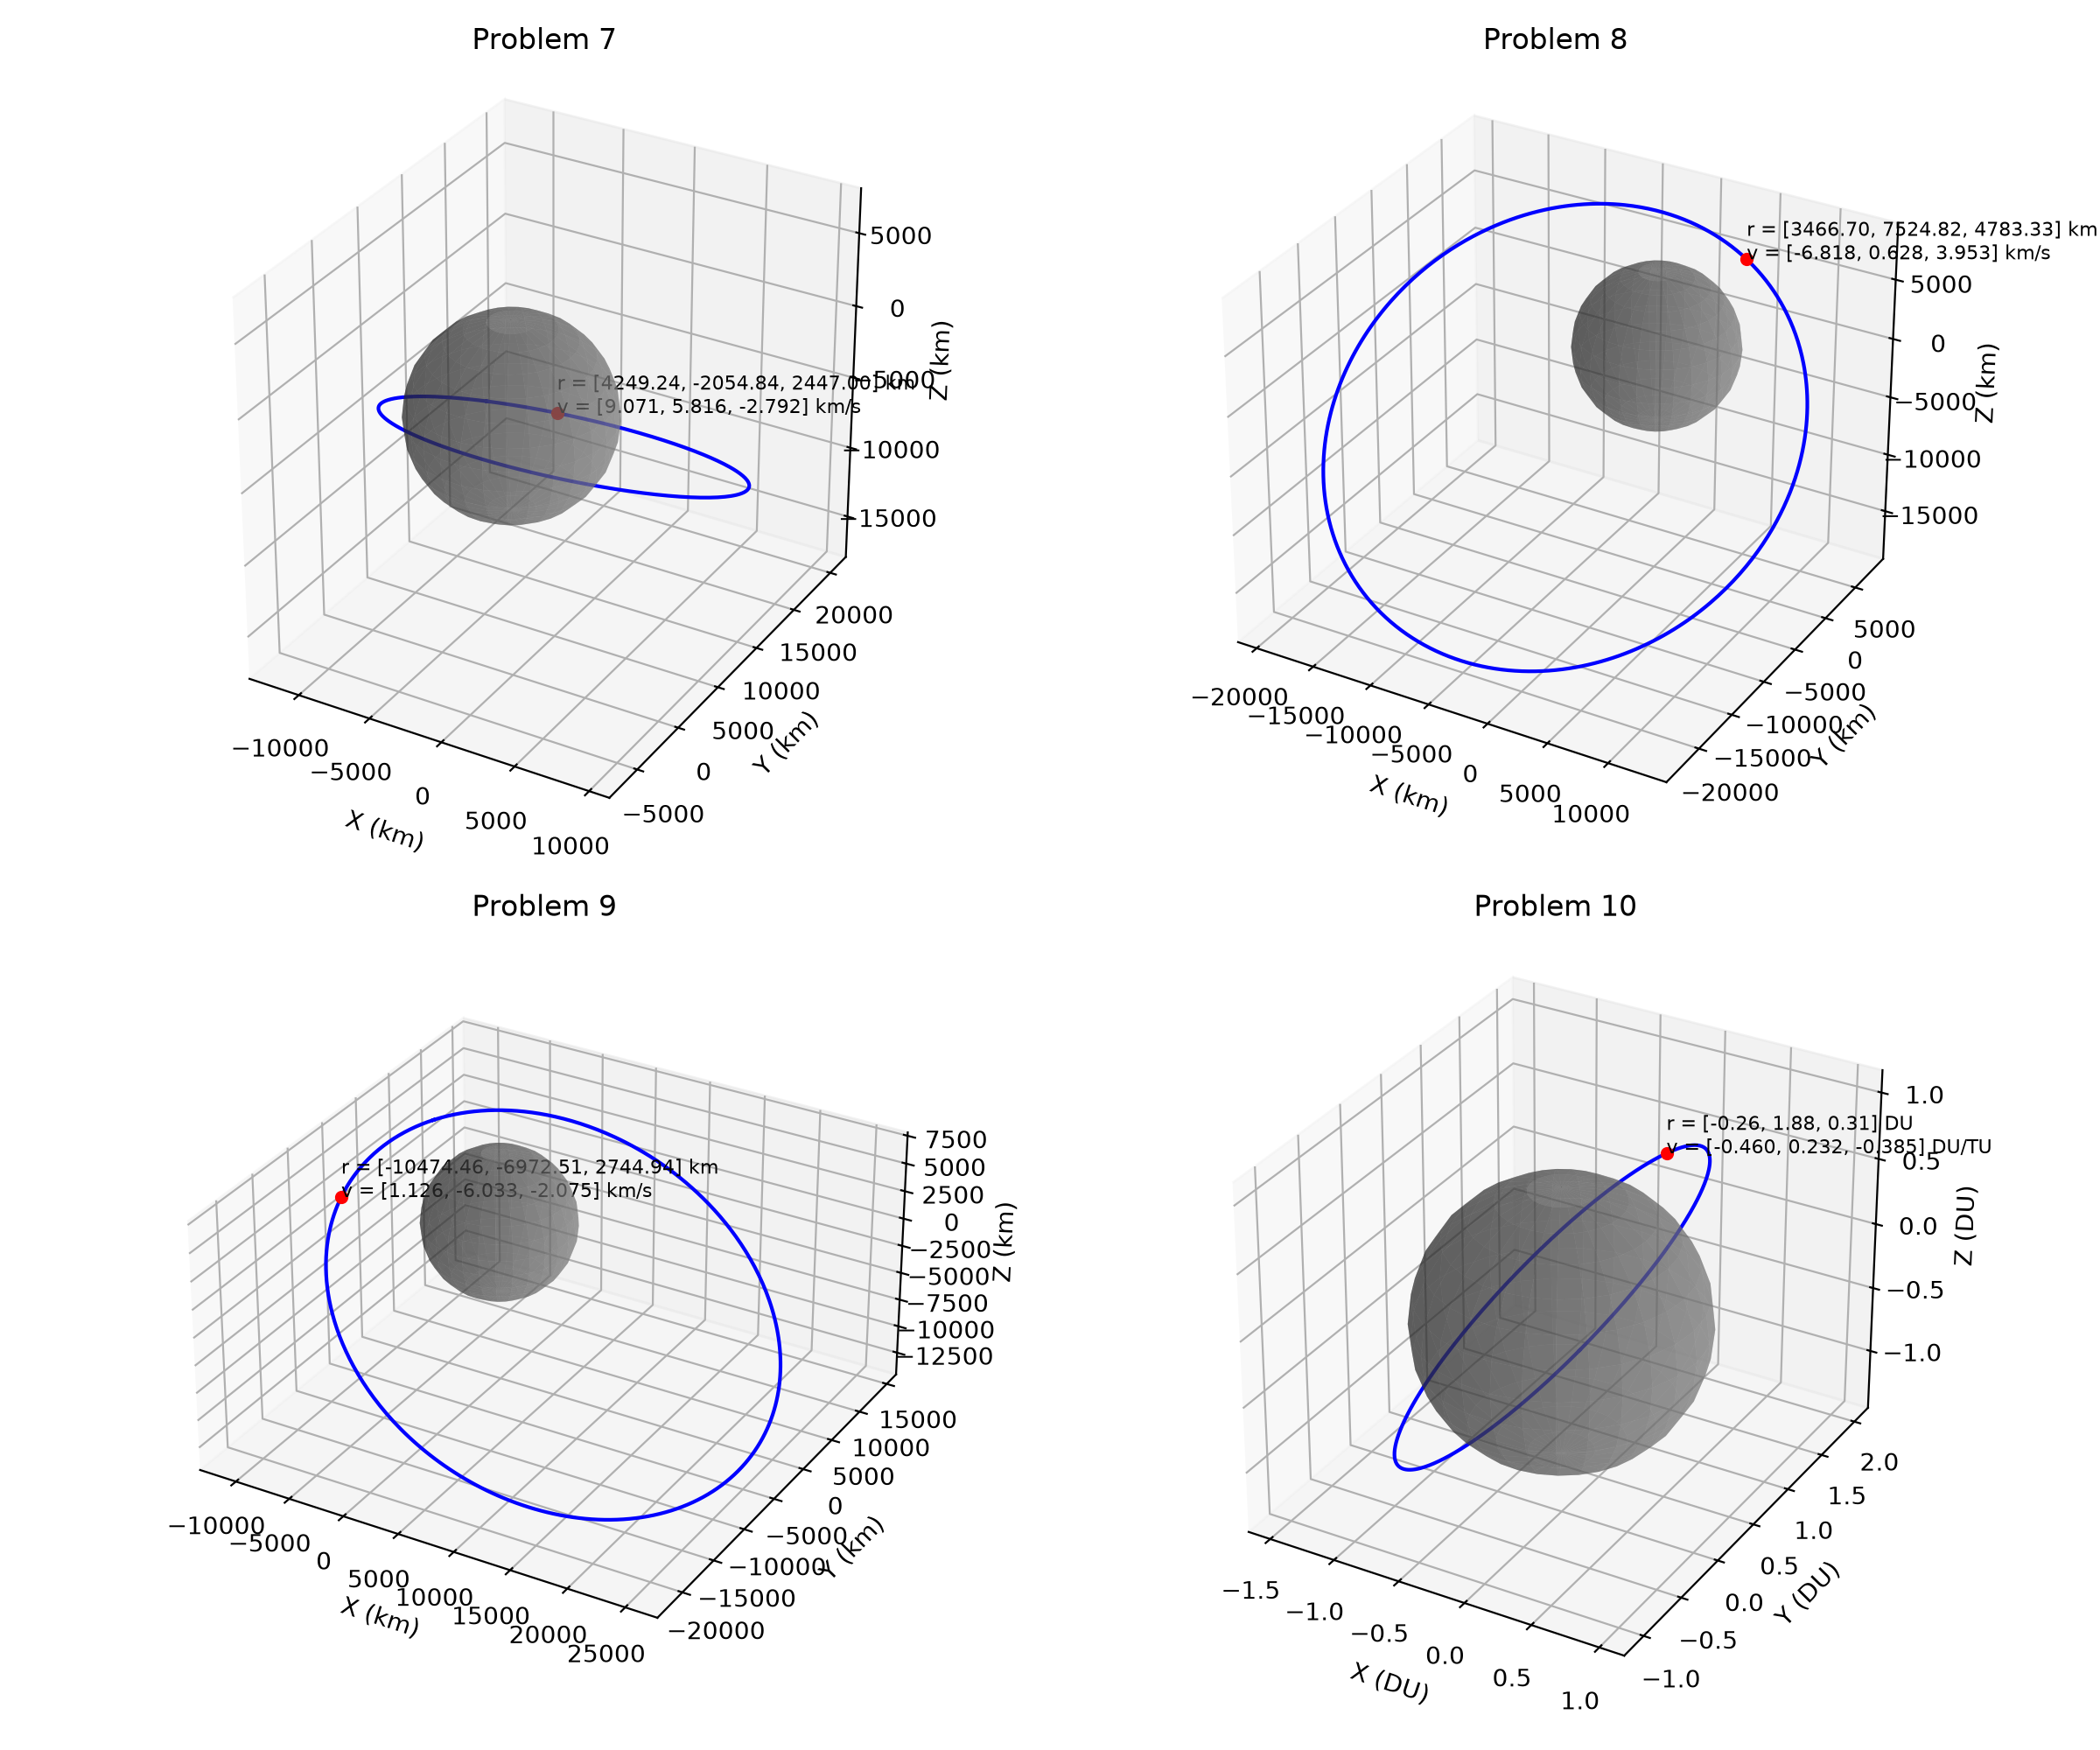
\includegraphics[width=\textwidth]{problems7to10_orbits.png}
\caption{Orbits for Problems 7 to 10 in planet-centered inertial coordinates. The planet (sphere of radius $R_E = 6378$ km, or 1 DU) is at the origin, and the spacecraft position (red) is labeled with its position and inertial velocity.}
\label{fig:p7-10}
\end{figure}

\FloatBarrier
